\begin{figure}[htbp]
\centering
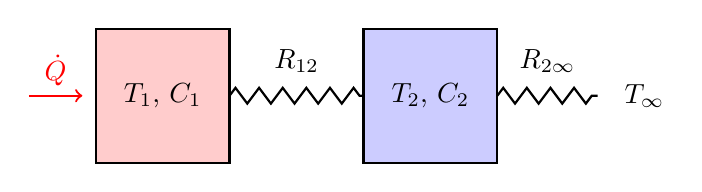
\begin{tikzpicture}[scale=0.85]
    % Body 1
    \draw[thick, fill=red!20] (0,0) rectangle (2,2);
    \node at (1,1) {$T_1$, $C_1$};

    % Body 2
    \draw[thick, fill=blue!20] (4,0) rectangle (6,2);
    \node at (5,1) {$T_2$, $C_2$};

    % Resistance between
    \draw[thick, decorate, decoration={zigzag, segment length=3mm, amplitude=1mm}]
        (2,1) -- (4,1);
    \node[above] at (3,1.2) {$R_{12}$};

    % Heat input
    \draw[->, thick, red] (-1,1) -- (-0.2,1) node[above, midway] {$\dot{Q}$};

    % Heat loss from body 2
    \draw[thick, decorate, decoration={zigzag, segment length=3mm, amplitude=1mm}]
        (6,1) -- (7.5,1);
    \node[above] at (6.75,1.2) {$R_{2\infty}$};
    \node at (8.2,1) {$T_\infty$};
\end{tikzpicture}
\caption{Two-capacitance thermal system.}
\label{fig:two_thermal}
\end{figure}
